% 关于intro的逻辑，我的一个八股文的经验写法（虽然老套，但是有用）：
% 第1段. 首先说自己的task是什么(如sequential rec、explainability、dro)，为什么重要（1-2句话)；然后引出related work，最好以上帝视角来总结related work的common paradigm，不是一个个简单工作的罗列；

% 第2段. 指出现有paradigm的limitation，必须佐以intuitive example/experiments + teaser figure；

% 第3段. 介绍key idea，注意是从idea层面来如何解决这个limitation的，结合第二段中的example和figure；

% 第4段. 介绍key tech，注意是从technical层面来介绍如何实现key idea的，最好以庖丁解牛的思维来写：分不同模块，每个模块核心tech是啥，为啥能解决limitation；

% 第5段. 介绍效果；

\section{Introduction}

Large language model distillation transfers capabilities from a stronger teacher to a smaller, more efficient student, aiming to reduce deployment costs while retaining reasoning, coding, and instruction-following abilities~\citep{alkhulaifi2021knowledge_kd}.
Conventional distillation uses teacher responses or token distributions on fixed contexts~\citep{yang2024kd_survey}.
At inference, however, the student conditions on its own prefixes and may encounter contexts poorly covered by offline supervision~\citep{gu2024minillm_opd,ko2024distillm_opd}.
On-policy distillation (OPD) mitigates this mismatch through a common loop: the current student generates rollouts, a teacher or evaluator supervises them, and the resulting signals guide student updates~\citep{song2026survey,lu2025onpolicydistillation}.
OPD methods vary by supervision interface, tokenizer compatibility, and granularity, with overlapping settings including logit-based distillation, cross-tokenizer alignment, self-OPD, black-box or rubric-based feedback, and step-wise or agentic supervision.


\begin{figure*}[t]
    \centering
    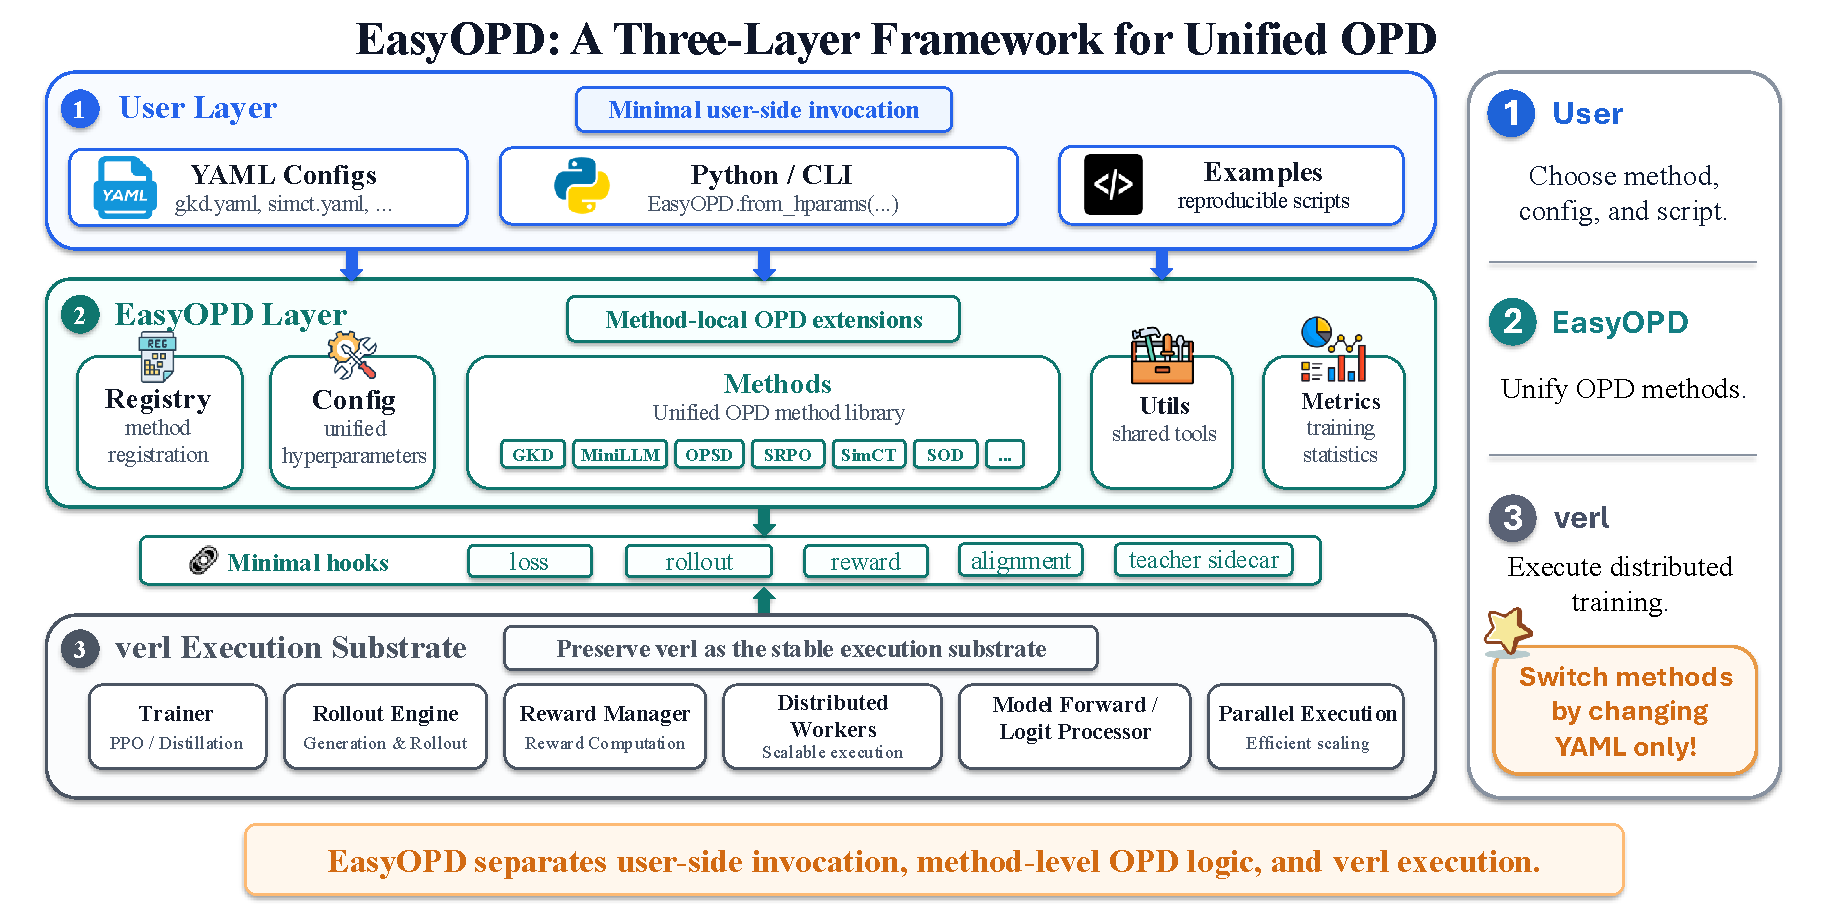
\includegraphics[width=1.0\textwidth]{figures/framework_0526.pdf}
    \caption{Architecture of \textsc{EasyOPD}. The user layer provides configuration-based invocation, the \textsc{EasyOPD} layer encapsulates method-local OPD logic, and verl provides distributed execution. Hooks for loss, rollout, reward, alignment, and teacher-side computation connect method modules to verl, allowing supported methods to share the same execution backend and be selected via YAML configurations.}
    \label{fig:framework}
\end{figure*}


A shared algorithmic paradigm does not yield a common system interface.
Depending on the supervision, OPD may span rollout generation, teacher inference, cross-tokenizer alignment, reward construction, distributed data flow, and optimization.
For example, cross-tokenizer OPD requires alignment or projection across teacher and student tokenizations before constructing compatible supervision, whereas black-box or rubric-based OPD may convert textual judgments or scores from a teacher or evaluator into rewards or training objectives; these supervision patterns therefore require different extension points.
Existing frameworks address complementary parts of the OPD workflow: TRL~\citep{vonwerra2020trl} provides trainer-centric distillation APIs; verl~\citep{sheng2024hybridflow_verl} and slime~\citep{slime_github} support scalable on-policy rollout and distributed execution; and KDFlow~\citep{zhang2026kdflow} provides a distillation-oriented stack.
However, as summarized in Table~\ref{tab:opd-frameworks}, we find no single reviewed framework that documents method-local extension boundaries across the heterogeneous supervision interfaces considered in this work while reusing a common distributed backend.
This gap calls for a lightweight OPD abstraction linking method-specific supervision to a shared execution substrate.


To fill this gap, we present \textsc{EasyOPD}, a unified OPD framework built on verl.
\textsc{EasyOPD} reuses verl for rollout generation, model execution, and optimization while adding a lightweight abstraction layer for method-local supervision.
Method modules connect to the shared training flow through explicit extension points: cross-tokenizer methods localize alignment and supervision construction, whereas black-box or rubric-based methods localize feedback acquisition and training-signal construction.
This design turns OPD integration from framework-wide modification into method-local extension.


To realize this design, \textsc{EasyOPD} adopts the three-layer architecture shown in Figure~\ref{fig:framework}. 
The user layer provides Python and CLI entry points and YAML configurations for specifying methods, teacher and student models, datasets, and hyperparameters.
The \textsc{EasyOPD} layer manages method registration, method-local modules, shared utilities, and supervision diagnostics.
Each module handles supervision acquisition, transformation, use, and diagnostics, and connects to verl through dispatch hooks for loss, rollout metadata, reward, alignment, and teacher-side computation.
The verl layer handles distributed rollout, model execution, worker orchestration, reward computation, and optimization.
Users select supported methods through configuration, while developers add methods by implementing and registering modules with the required hooks. For the evaluated implementations, method-specific supervision logic is placed in registered method-local modules, and the core trainer and workers interact with them only through the shared dispatch layer.
Through these layers, we implement and evaluate representative methods across three settings: cross-tokenizer OPD, on-policy self-distillation, and step-wise OPD. The framework also implements logit-based OPD, and its extension boundaries are designed to accommodate additional supervision forms such as black-box or rubric-based feedback.


We evaluate \textsc{EasyOPD} through three case studies covering cross-tokenizer OPD, on-policy self-distillation, and step-wise OPD.
Within each setting, methods share the model initialization, training data, execution backend, and evaluation procedure where applicable, while retaining their original supervision designs.
Once the shared hook layer is in place, each evaluated method concentrates its supervision logic in a small set of registered method-local files and reuses the existing dispatch sites in the core rather than introducing new method-specific components; we report the per-method integration cost in Section~\ref{sec:experiments}.
We further report framework overhead relative to matched verl runs in Section~\ref{sec:experiments}, separating teacher-inference, alignment, and reward-evaluation costs from the dispatch layer itself.
We release the code under the Apache License 2.0 on GitHub with reproducible YAML configurations, documentation, and an installable demonstration package with runnable examples.
